%=========================================================================
% (c) Michal Bidlo, Bohuslav Křena, 2008

\newtheorem{definice}{Definice}

\chapter{Úvod}\label{uvod}
	Výškoměr je jedním z nepostradatelných přístrojů pro navigaci za letu. Je důležité aby fungoval správně ve~všech situacích, jelikož~chyba v~měření může znamenat havárii letadla. V~lepším případě dojde "pouze" ke~škodám na~majetku, v~horším případě může dojít i~ke~ztrátám na~životech. Plní nezastupitelnou úlohu, díky níž mohou piloti bezpečně létat i~za~špatné viditelnosti.
	
	\section{Motivace}\label{uvod::motivace}
		Motivace pro tuto práci je zvýšení bezpečnosti a~ulehčení výcviku začínajících pilotů. Jde hlavně o~ulehčení výuky přistání, která začátečníkovi může způsobovat potíže. Jedná se primárně o~výuku dosednutí(anglicky "flare"), kdy musí student stáhnout výkon motoru a~přitáhnutím uvést letoun do~horizontálního letu, ideálně několik centimetrů nad dráhou. Student pomalu přitahuje knipl, tímto~zvyšuje úhel náběhu a~letadlo postupně zpomaluje. V~okamžiku, kdy je úhel náběhu příliš velký a~rychlost letadla moc nízká, křídla ztratí vztlak a~letadlo dosedne na dráhu. Pokud student udržuje letadlo v~horizontálním letu nad dráhou ve~velké výšce, může být dosednutí tvrdší, než na~které~je stavěn podvozek, a~může dojít k~poškození podvozku či~zranění posádky i~cestujících.
	
	\section{Cíle}\label{uvod::cile}
		Prvním cílem této práce je úvod do~problematiky týkající se~radarů. Čtenáři budou přiblíženy rozdíly mezi jednotlivými typy radarů, principy jejich fungování a~technologiemi, které za~nimi stojí. Druhým cílem je popis problému výuky přistání a~důvod pro zadání této práce, jakožto i~jejího řešení. Třetím cílem je návrh takového systému, který~splní veškeré požadavky na bezpečnost letového provozu na letištích, zvýší bezpečnost výuky přistání a~samozřejmě zjednoduší samotnou výuku. V neposlední řadě je samotná implementace již zmíněného systému a~jeho integrace do letadla. Nakonec je třeba systém jako celek otestovat a~zajistit, že bude bezchybně fungovat za~jakýchkoliv podmínek. V~případě, že bude systém funkční, je možnost jej rozšířit a~aplikovat v~komerční praxi. 

\chapter{Historie}
	\section{Vývoj přístrojů}
	
		V roce 1903 bratři Wrightové uskutečnili první řízený motorový let. Trval jen chvíli, ale~byl to~přelom v~technologii dopravy. Tímto začala éra letectví. Za první světové války, kdy došlo k~prvnímu masivnímu rozšíření letadel,  ať~již k~průzkumným účelům, bombardování nebo~vzdušným soubojům byli piloti omezeni počasím a~za špatného počasí nemohli létat, jelikož neexistovala technologie, která by umožnila pilotovi nespoléhat pouze na svůj zrak a~navigovat za letu i~jinak, než~pouze vizuálně. Toto vedlo ke~snahám vyvinout systém, který~by~umožňoval navigaci za~jakýchkoliv podmínek. Za~jasného slunečného počasí nebo třeba v~bouřce.\par
		
		Začaly se objevovat první přístrojové desky a na nich první přístroje. Kvůli omezené ploše palubní desky se na ni moc přístrojů nevlezlo, proto na ni bylo umístěno pouze několik nejdůležitějších přístrojů. Mezi tyto přístroje patřil kompas, teploměr oleje, otáčkoměr, ukazatel indikované rychlosti a~samozřejmě výškoměr. S tímto primitivním vybavením se museli spokojit piloti během první světové války i v období míru po ní. Postupem času toto omezené vybavení přestalo splňovat podmínky pro přístrojové lety a s nástupem nových technologií se na palubní desku muselo vejít mnohem více zařízení. Každé letectvo prodělalo vývoj, bohužel, nejrychlejší byl v dobách druhé světové války, kdy došlo k nejrychlejšímu technologickému pokroku na obou stranách. Rozdíl mezi přístrojovými deskami jednotlivých národů můžeme pozorovat na obrázcích \ref{historie::vyvojPristroju::kokpitG2} a~\ref{historie::vyvojPristroju::kokpitP51}.
		Podoba kokpitu se podstatně neměnila až do příchodu digitální technologie, kdy analogové přístroje nahradily sofistikované systémy zobrazující veškeré údaje potřebné pro všechny fáze letu a v případě vojenských letounů i pro bojové situace na displeje v kokpitu. 
		
		\begin{figure}[H]
			\begin{center}
				\includegraphics[scale=0.42]{obrazky-figures/G2_dashboard.jpg}
				\caption{Přístrojová deska stíhacího letounu Bf109-G2\protect\footnotemark}\label{historie::vyvojPristroju::kokpitG2}
			\end{center}
		\end{figure}
		\footnotetext{zdroj: \url{http://forum.largescaleplanes.com/index.php?showtopic=8725}}
	
		\begin{figure}[H]
			\begin{center}
				\includegraphics[scale=0.4]{obrazky-figures/P51-cockpit-1000.jpg}
				\caption{Kokpit doprovodného stíhacího letounu P51\protect\footnotemark}\label{historie::vyvojPristroju::kokpitP51}
			\end{center}
		\end{figure}
		\footnotetext{zdroj: \url{http://www.warbirdalley.com/p51.htm}}
		
		
	\section{Vývoj měření výšky a úvod do této problematiky}
	
		Barometry byly lidstvu známy již od~17. století, tyto bohužel obsahovaly vodu. Aby mohl být tlak vzduchu úspěšně změřen, barometr vyžadoval přibližně 10 metrů vysokou trubici. Avšak italskému matematikovi a~fyzikovi Evangelistovi Torricellimu se podařilo zkrátit délku trubice na 80cm nahrazením vody rtutí, která je cca třináctkrát hustší než voda. I přes své relativně malé rozměry je tento barometr pořád příliš velký pro masové rozšíření. Za další zmenšení přístroje je zodpovědný francouzský vědec Lucien Vidi, který vynalezl aneroidní barometr, přezdívaný aneroid\cite{history::aneroid}.\par
		Díky této změně se barometr zmenšil na rozumnou velikost a již se dal použít v omezeném prostoru letadel. Ve skutečnosti je barometrický výškoměr pouze překalibrovaný aneroid. Bohužel stejně jako ukazatel indikované rychlosti je závislý na mnoha faktorech. Mimo jiné můžeme jmenovat teplotu a vlhkost vzduchu. Zásadním problémem je, že barometrický výškoměr už z principu neukazuje relativní výšku nad terénem, ale výškud AMSL(height Above Mean Sea Level). Reálně tedy dvě letadla letící podle výškoměru ve výšce 6000 stop několik desítek námořních mil od sebe mohou být v jiné nadmořské výšce. Na obrázku \ref{historie::vyvojMereniVysky::FL} je názorná ukázka. Zde může čtenáře napadnout, zda se letadla kvůli rozdílným indikovaným hodnotám nesrazí. Barometrické výškoměry sice ukazují nadmořskou výšku špatně, ale když se letadla přiblíží, tak ukazují stejně špatně a letadla se tedy minou.\par
		\begin{figure}[H]
			\begin{center}
				\includegraphics[scale=0.75]{obrazky-figures/flight_level.png}
				\caption{Rozdíl mezi barometrickou(nadmořskou) výškou a aktuální výškou}\label{historie::vyvojMereniVysky::FL}
			\end{center}
		\end{figure}
				
		Další potíže nastávají s rozdílnými atmosférickými tlaky mezi počátečním a cílovým letištěm. Mějme následující situaci: Letadlo letí z letiště Shiphol v Amsterdamu, které je tři metry pod hladinou moře, do Himalájí. Zde se v Tibetu nachází letiště Bangda ve výšce 4334 metrů\cite{bangda}. Rychlou úvahou dojdeme k závěru, že  si pilot bude muset dávat pozor v jaké výšce nad terénem letí a na jakou výšku bude přistávat. Toto bylo vyřešeno přidáním možnosti kalibrace. Pilot před vzletem nastaví hodnotu QNH, kterou pilotovi sdělí řídící letového provozu, taktéž před přistáním učiní řídící v cílové oblasti. Na obrázku \ref{historie::vyvojMereniVysky::109Altimeter} můžeme vidět bíle okénko ukazující tlak QNH a kolečno pro jeho nastavení. Do přechodové hladiny se používá tento výškoměr a nad touto hladinou pilot letí podle druhého výškoměru, který je pevně nastaven na hodnotu 1013.25 hPa. Toto je pevně zavedený standard pro veškeré civilní lety. 
		
		\begin{figure}[H]
			\begin{center}
				\includegraphics[scale=0.75]{obrazky-figures/109Altimeter.jpg}
				\caption{Výškoměr z letounu Bf109\protect\footnotemark}\label{historie::vyvojMereniVysky::109Altimeter}
			\end{center}
		\end{figure}
		\footnotetext{zdroj: \url{http://www.warbirdsite.com/Collection.html}}
		
	
%	\paragraph{Existující radarové výškoměry}
%	Radarové výškoměry nejsou žádná novinka. Dnes jsou využívány v~letectví ale i~pro vědecké účely.
%	V letectví jsou hlavní součástí GPWS(Ground Proximity Warning System) kde~se používá jako absolutní výškoměr(měří vzdálenost letadla od~zemského povrchu). Teto systém byl rozšířen na Enhanced Ground Proximity Warning system, který~již spolupracuje s~celosvětovou digitální databází povrchu Země.
%	Pro vědecké účely jsou využívány v~případě husté atmosféry pro skenování povrchu(např. Venuše nebo Země)
	
	\section{Vývoj radaru}
		Zrození radaru se datuje do počátku 20. století, kdy~si mocnosti nezávisle na~sobě uvědomily význam této technologie. Mezi lety 1934 a~1939 začaly USA, Velká Británie, Německo, Sovětský svaz, Japonsko, Nizozemsko, Francie a Itálie nezávisle na sobě vyvíjet systém detekce pomocí radiových vln.\cite{history::radar} Vývoj radaru výrazně pomohl při~bitvě o~Británii, kdy~britové detekovali formující se letadla Luftwaffe nad Francouzským územím, a~tímto umožnil rychlou odezvu Britských pilotů.\par
			
		Během studené války se radary výrazně zdokonalily. Zvětšil se jejich výkon a~zmenšila se jejich velikost. V současné době se radary houfně využívají k~mírovým účelům, od~sledování počasí přes letectví či~posuny zemské kůry až po mapování.
\chapter{Teoretická část}
	
	\section{Radary a jejich dělení}\label{uvod::radary}
		Radar (\textbf{RA}dio \textbf{D}etection \textbf{A}nd \textbf{R}anging) je systém detekce objektů, který~je pomocí rádiových vln určit vzdálenost, azimut a rychlost sledovaných objektů. Využití radarů je široké, od~mapování terénu, detekce osob přez měření rychlosti vozidel a~využití v ~civilním letectví až~po~vojenské účely.	
			
	\paragraph{Klasifikace radarů}
			Radary se dělí podle typu vysílání a~podle použití\cite{radarClasification}. Základní dělení je: 
			\begin{itemize}
				\item \textbf{Primární radar}	-	Slouží k zobrazování předmětů. Vysílač vysílá vysokofrekvenční signál a~příjmač zachytává ozvěnu vysílaného signálu.
					
				\item \textbf{Sekundární radar}	-	Slouží k přenosu informací. Aby toto spojení fungovalo, musí mít cílový objekt zapnutý transpondér, který~po přijetí signálu zpracuje dotaz a~odpoví požadovanými informacemi např. výška, rychlost, souřadnice GPS a kurz. 
			\end{itemize}
			
			Primární radary se dále dělí na:
			\begin{itemize}
				\item \textbf{Pulsní}	-	Tomuto typu radarů postačuje pouze jedna anténa a~to z~toho důvodu, že~se radar periodicky přepíná mezi vysílacím režimem a příjmacím režimem. Z tohoto pramení nevýhoda tohoto typu radarů: minimální dosah. Minimální dosah radaru je určen rychlostí přepínaní mezi jednotlivými režimy. Pokud se vrátí ozvěna dříve, než~se radar přepne do~příjímacího režimu, radar objekt nedetekuje a~informace je ztracena.
				
				\item \textbf{Kontinuálně vysílající}	-	Radary tohoto typu vysílají nepřerušovaně a~zároveň nepřerušovaně zpracovávají přijatou ozvěnu. Tyto radary se dělí na:
					\begin{itemize}
						\item Modulované - Tyto radary využívají frekvenční modulace signálu, díky které jsme schopni vypočítat vzdálenost z~ozvěny vysílaného signálu. Toto je typ radaru, se~kterým~budeme pracovat v této práci.
						
						\item Nemodulované - Tyto radary vysílají konstantní signál, který~umožňuje pouze určení rychlosti zachycených objektů.
					\end{itemize}
			\end{itemize}
		
		\section{Vestavěné systémy}
			Jelikož náš systém má jedinný účel: zjistit výšku letadla nad přistávací dráhou, využívat víceúčelová zařízení je pro~nás zbytečně robustní a~neforemné. Potřebujeme jednoduché, rychlé a~elegantní zařízení, které~bude plnit pouze jedinný úkol. Zde přicházejí do hry embedded systémy.
			
			\begin{definice}
				Vestavěné systémy VS jsou systémy, ve~kterých~je zpracování dat vestavěno/vloženo do~většího systému a~ve~kterém není zpracování dat viditelné uživateli prostřednictvím např. PC počítače. Anglicky se vestavěné systémy označují jako \textbf{embedded system}\cite{impSkripta}.
			\end{definice}
			
			Embedded zařízení je jednoduchý a~elegantní způsob řešení jednotvárných algoritmických úloh. Naše úloha musí být vykonávána v~reálném čase, tzn. máme určenou dobu odezvy a~tu musíme splnit. Nutnost mít co nejnižší odezvu určuje nároky na~zvolené zařízení. Na tomto zařízení poběží pouze jedinná aplikace. To nám umoňuje optimalizovat aplikaci na~míru systému pro dosažení co~největšího výkonu.
			Bohužel optimalizace aplikace není vše. Aby se algoritmus vykonával co~nejrychleji, musíme pro ni~zvolit odpovídající zařízení. Pro náši aplikaci potřebujeme zajistit dostatečně rychlé vzorkování abychom zabránili aliasingu. Toto je nejlepší řešit na~hardwaru, jelikož rychlost zpracování bude vyšší a~budeme schopni zaručit splnění podmínky Nyquistova teorému, kdy~vzorkovací frekvence musí být alespoň dvakrát větší než~maximální frekvence signálu: \[f_v > 2f_{max}\]
			
			Pro tuto úlohu se hodí programovatelné hradlové pole FPGA. Toto pole nám bude vzorkovat signál s~dostatečnou frekvencí a~po sběrnici jednotlivé vzorky posílat dále do procesoru pro zpracování.\par
			
			\paragraph{Xilinx Zynq}
				Po určení požadavků na~hardware v~ůvahu připadají zařízení od~výrobce programovatelných hradlových polí Xilinx. Konkrétně rodina procesorů Zynq, která~kombinuje FPGA s~procesorovým jádrem ARM Cortex.
				Jak již bylo zníněno výše, FPGA navzorkuje signál a~pošle jej k~dalšímu zpracování přez AXI porty jádru procesoru ARM, na kterém poběží odlehčená verze Linuxu. Na tomto operačním systému poběží aplikace provádějící potřebné výpočty a~bude posílat výsledek na výstup.
				
				\begin{figure}[h]
					\begin{center}
						\includegraphics[scale=0.6]{obrazky-figures/zynq-mp-core-single.png}
						\caption{Architektura procesoru Zynq-7000\protect\footnotemark}
						\label{teorie::embedded::zynq}
					\end{center}
				\end{figure}
				\footnotetext{zdroj: \url{https://www.xilinx.com/products/silicon-devices/soc/zynq-7000.html}}
			
			\paragraph{Řídící modul}
				Řídící modul obsahující výše zmíněný procesor je dodán společností CAMEA s.r.o. Modul obsahuje vstupně výstupní porty , které~můžeme využít v~náš prospěch. Jako výstupní porty můžeme využít USB sběrnici s~přímým přístupen do paměti, GPIO porty nebo Serial Peripheral Interface. 
				\begin{itemize}
					\item USB můžeme využít pro přenos přesných informací obrazovou formou na displej, kde zobrazujeme výšku. Formát by mohl být následující: \[ALTITUDE = 10.0 m\]\[ALTITUDE = 33 ft\]
					
					\item Pomocí GPIO portů, případně rozhraní SPI, můžeme ovládat panel s LE Diodami, který~barevnými LED seřazenými vertikálně. Tento panel bude mít diody vyzařující světlo od~zeleného spektra, přes žlutou, oranžovou a~sytě červenou, kdy~bude začínat fáze dosednutí.
					
					\item Zvuková komunikace může probíhat generováním tónů a~odesílání konektorem typu 3.5mm Jack. Bude se generovat stále stejný tón konstantní délky, přičemž zkracující se perioda bude signalizovat snižující se výšku. Pokud bude letadlo těsně nad zemí, bude se generovat tón bez přerušení.
				\end{itemize}
			
			\paragraph{Kalibrace modulu}
				Další částí naší úlohy je nutnost kalibrace zařízení, jelikož každé letadlo může mít tento modul umístěno v jiné výšce nad zemí. Kalibrace může být statická - v kódu bude přičtena konstanta, nebo dynamická, kdy~se před startem modul zkalibruje. Statická kalibrace má výhodu jednoduššího chování modulu a~bude vyžadovat o~jeden ovládací prvek méně, avšak bude nutno zasahovat do zdrojových kódů při instalaci na jiné letadlo. Dynamická kalibrace, na rozdíl od~statické, má nevýhodu složitějšího řídícího programu, ale~je bude možno mít jeden program pro všechny typy letadel. Přidaný ovládací prvek nebude téměř znát. V tomto případě se autor přiklání k~dynamické kalibraci.
				
			\paragraph{Ovládací panel}
				Nutnost kalibrace nás přivádí k~ovládacímu panelu modulu. Přístroj je třeba nějak zapnout, toto bude první přepínač. Dále vyvstává otázka nutnosti mít vždy zapnutou zvukovou signalizaci. Jelikož bude využití tohoto výškoměru při vzletu mizivé, bude dobré, když~bude mít pilot možnost vypnout zvukovou indikaci, která~v~situaci, kdy~ji není potřeba může působit rušivě. Proto může být přítomen přepínač ovládající tuto funkci. Jako třetí kontrolní prvek zvolíme tlačítko spouštějící kalibraci přístroje na referenční hodnotu země. Je nutné, abychom zabránili kalibraci výškoměru ve vzduchu, proto by mělo toto tlačítko být překrité víčkem. V případě, že~bude koncipováno jako ovládací prvek na dotykovém displeji, za~pohybu letadla by mělo být deaktivované.
				
	\section{Fáze přistání}
		Letadlo, které~vzlétne, se musí dostat zpět na~zem rozumným a~hlavně bezpečným způsobem. Není žádoucí aby letadlo i~pasažéři byli na jedno použití. Bezpečné přistání je nejdůležitější fází letu.\par
		Když se blíže podíváme na přistání, je to doslova řízený pád. Letadlo ztrácí výšku a~rychlost aby~bezpečně dosedlo na zem a~je zde malý prostor chybovat. Proto je kladen velký důraz na výuku a~správné naučení přístávání. Přistání lze rozdělit do několika fází\cite{landingPhases}:
			
		\begin{enumerate}
			\item Závěrečné přiblížení (Final approach) - Během této fáze pilot musí udržovat přibližovací rychlost danou výrobcem letadla a~letět po kurzu osy dráhy pod sklonem určeným přibližovacími pravidly(glidepath).
					Během této fáze pilot uvádí letoun do přistávácí konfigurace.
					
					\item Výběh (zeptat se prof Zemcika na spravny cesky preklad Flare) - Když se pilot přibližuje k~dráze, musí přitáhnout knipl, tím zvýší úhel náběhu a~zpomalení stroje. Letadlo je závislé na rychlosti proudění vzduchu okolo křídel. Když je proud vzduchu příliš pomalý a~úhel náběhu nestíhá kompenzovat ztrátu vztlaku, letadlo se dostane do pádu. Pilotovým úkolem v~této fázi letu je s~vypnutým motorem udržovat letadlo ve vodorovném letu těsně nad dráhou, na kterou~pak dítky ztrátě vztlaku dosedne. Je důležité, aby letadlo bylo těsně nad dráhou, čím výše se v~okamžiku ztráty vztalu letadlo nachází, tím tvrdší přistání může čekat.
					
					\item Dosednutí a~rolování (Touchdown and taxi) - Po dosednutí pilot zpomalí letadlo na požadovanou rychlost pro rolování a~roluje na místo určené řídícím na věži. 
				\end{enumerate}
				
				
			
\chapter{Návrh řešení}\label{navrhReseni}
	Radarový výškoměr zpracovává vstupy zcela automaticky bez zásahu uživatele(pilota) a~uživateli pouze zobrazuje zpracované výsledky. Uživatel vůbec nepotřebuje vědět, co a~jak funguje, stačí mu pouze zobrazená výška. Vzhledem k~omezenému prostoru, kam~letadlo umožňuje instalovat další zařízení, jsme nuceni vyhledat co nejmenší řešení, které~je ale~zároveň dostatečně výkonné, aby~v~reálném čase zvládalo zpracovávat signály a~převést výsledky do vhodné formy pro rychlé a~správné vyhodnocení pilotem.
	
	\section{Platforma}\label{navrhReseni::platforma}
		Jak již bylo zmíněno v~úvodu této kapitoly, potřebujeme malé, ale~rychlé zařízení, které bude v~reálném čase poskytovat údaje o~aktuální výšce. V našem případě, vzhledem k~reakční době člověka cca půl sekundy, bude stačit, když systém stihne spočítat výsledek a~předat jej pilotovi do $\sim$250ms.\par
		
		Kvůli nárokům na velikost můžeme vyřadit objemné osobní počítače a~spíše se ponořit do~oblasti embedded systémů. V~současnosti trh nabízí dostatečně výkonné a~zároveň dostatečně kompaktní zařízení, která~jsou pro náš účel vhodná. Jako možný kandidát se jeví mikropočítač Raspberry Pi, který už je dostatečně výkonný a~zároveň malý aby mohl plnit naši úlohu. Vhodnější alternativa k~tomuto řešení se jeví procesor rodiny Zynq od~výrobce Xilinx, který je určen přesně pro naše potřeby, a~díky hradlovým polím FPGA výrazně urychluje zpracování ozvěny signálu. Přístroj s~procesorem dodala společnost CAMEA s.r.o.
	\section{Radar}
		Radarový transciever, se~kterým~budeme v~této práci pracovat je K-MC1 Radar Transciever firmy RFbeam Microwave GmbH. Jedná se o kontinuálně vysílající a~příjmající radar s~frekvenční modulací. Díky frekvenční modulaci vysílaného signálu jsme schopni změřit nejenom rychlost objektu, ale~i~jeho vzdálenost, což je pro naše účely perfektní.
	
		
	\section{Výstupní zařízení}
		Náš systém musí s~pilotem nějak komunikovat. Způsob komunikace musí být tak detailní, aby dokázal předat informace o~výšce nad~zemí a~zároveň dostatečně jednoduchý, aby pilot mohl data ze~systému zpracovat rychle a~efektivně aniž by výstupní zařízení odklánělo pozornost od~právě prováděných úkonů. Jedna z~možností je použití zvukových signálů, druhá je zobrazování aktuálních informací na displej. Autor se rozhodnul pro kombinaci obou způsobů. Zvukové signály umožní věnovat pozornost ději v~okolí letadla aniž by vyrušovaly pilota, pro podrobnější informace se bude moct podívat na displej.
			
	\section{Software}\label{navrhReseni::software}
		
		TODO %Poznamky autora, prosim nezlobte se. Linux, na kterem pobezi program tahajici data z radaru a pocitajici vyslednou vysku a rychlost, nutna konzultace na vystup zarizeni a testy co za cisla z toho vubec lezou, vysledek hratek s matlabem by se dal klasifikovat jako: meh. keywords: Hammingovo okno, 50\% prekryti vzorku => prace s poli => kastliku jak nasranych => program bude giganticky zrout pameti. Zjistit, jestli existuje knihovna pro praci se signaly v C at to nemusim prasit ja, bylo by to nefektivni a pomale.
	
	\section{Umístění na letadle}\label{navrhReseni::umisteniNaLetadle}
		Zařízení musí být na~letadle umístěno tak, ať~je šance požkození přístroje při tvrdším přistání minimální a~zároveň musí být měření konzistentní. Toto vylučuje umístění přístroje na~konci křídel. Může dojít k~odření křídla o~zem při přílišném naklonění, navíc bude muset být provedena velká korekce výšky a~může dojít k~změnám detekované výšky při náklonech letadla, taky dojde k narušení aerodynamického tvaru křídla. Ideální by bylo umístit senzor na pneumatiky jednoho z~kol hlavního podvozku, bohužel velice rychle zjistíme, že~je to nevhodné řešení z~důvodů jednorázového použití radaru. Jako vhodné možnosti se jeví umístění:
		\begin{itemize}
			\item na~nohu podvozku za předpokladu, že~se na~ni zařízení vejde(v případě zatažitelného podvozku). Při umístění na~pevný podvozek je třeba zamezit možnosti vzniku poškození následkem otřesů při tvrdém přistání. 
			\item na~spodní část kořene křídla, kde~nebude moment síly způsobující rotaci letadla ve~vodorovné ose tak velký, jako na konci křídla. Otřesy, které~bude muset zařízení snášet nebudou tak velké jako na noze hlavního podvozku. Bohužel zde zůstává nutnost korekce podle výšky kořene letadla nad~rovinou podvozku.
			\item na trup letadla, toto bohužel bude vyžadovat vrtání do trupu a~tudíž úpravu konstrukce letadla.
			\item do trupu letadla, ideálně do~odpružené schránky s~dvířky, která by se otevřela při spuštění radaru při náletu na přistání. Opět zde je otázka modifikace konstrukce letadla.
		\end{itemize} 
		Note: Asi bude nejlepší přilepit to na nohu, ať nemusíme vrtat, to je třeba zkonzultovat s majitelem letadla. Ostaní možnosti jsou příliš drahé.


%=========================================================================
